% ===============================================================================
% = LaTeX Beamer Template des Arbeitsbereichs Sicherheit in verteilten Systemem
% = (c) 2012 Prof. Dr. Hannes Federrath, Uni Hamburg, Fachbereich Informatik
% = http://www.informatik.uni-hamburg.de/svs/
% ===============================================================================
%
\documentclass[t, aspectratio=169]{beamer} 
% Option t              Place text of slides at the (vertical) top of the slides.
% Option handout        Ein PDF ohne Pausen und Overlayeffekte erzeugen.
% Option aspectratio=43 169 => 16:9, 1610 => 16:10, 43 => 4:3
\usepackage[utf8]{inputenc}
%\usepackage[ngerman]{babel}
\usepackage{graphicx,xcolor}
\usepackage[T1]{fontenc} % 8-Bit-Zeichen; ermöglicht korrektes Kopieren von Umlauten aus dem pdf 
\usepackage[scaled]{helvet}

\usepackage{beamerthemedefault}

% Ränder definieren
\setbeamersize{text margin left=5ex, text margin right=5ex}

% Farbdefinitionen
\definecolor{svsgrau1}{RGB}{191,191,191} % Balken in Kopfzeile
\definecolor{svsgrau2}{RGB}{123,123,123} % Folienüberschriften
\definecolor{svsrot}{RGB}{255,0,0} % Bullets
\definecolor{svshellblau1}{RGB}{153,204,255} % Block Hintergrund
\definecolor{svshellblau2}{RGB}{24,113,248} % Anstrich Ebene 2
\definecolor{svsdunkelblau}{RGB}{38,82,128} % Text der Ebene 1

% Navigationsleiste ausblenden
\beamertemplatenavigationsymbolsempty 

% Farben der Bullets der Ebenen
\setbeamercolor{itemize item}{fg=svsrot}
\setbeamercolor{itemize subitem}{fg=svshellblau2}
\setbeamercolor{enumerate item}{parent=itemize item}
\setbeamercolor{enumerate subitem}{parent=itemize subitem}

% Formen der Bullets der Ebenen
\setbeamertemplate{itemize item}[circle] 
\setbeamertemplate{itemize subitem}{--} 
\setbeamertemplate{itemize subsubitem}[circle] 

% Farben der Texte 
\setbeamercolor{title}{fg=black}
\setbeamercolor{structure}{fg=svsgrau2}
\setbeamercolor{section in toc}{fg=black}
\setbeamercolor{framesubtitle}{fg=svsdunkelblau}
\setbeamercolor{itemize/enumerate body}{fg=svsdunkelblau}
\setbeamercolor{itemize/enumerate subbody}{fg=black}
\setbeamercolor{itemize/enumerate subsubbody}{fg=black}

% Zeichensätze der Texte
\setbeamerfont{author}{size=\normalsize}
\setbeamerfont{institute}{size=\normalsize}
\setbeamerfont{date}{size=\normalsize}
\setbeamerfont{frametitle}{size=\large}
\setbeamerfont{framesubtitle}{size=\footnotesize\raggedleft}
\setbeamerfont{sections/subsections in toc}{size=\normalsize}
\setbeamerfont{itemize/enumerate body}{size=\normalsize}
\setbeamerfont{itemize/enumerate subbody}{size=\normalsize}
\setbeamerfont{itemize/enumerate subsubbody}{size=\normalsize}

% Definitionen für farbig hinterlegten Block 
\setbeamertemplate{blocks}[rounded]
\setbeamercolor{block title}{fg=black,bg=svshellblau1}
\setbeamercolor{block body}{parent=normal text,use=block title,bg=block title.bg!25!bg}
\setbeamerfont{block title}{size=\normalsize}
\setbeamerfont{block body}{size=\normalsize}

% Definitionen für Agenda (FIXME: noch stärker an normale Listendefs. anpassen)
\setbeamertemplate{section in toc}[sections numbered]
\setbeamertemplate{subsection in toc}[square]

% Kopfzeile
\setbeamertemplate{headline}{
	
\includegraphics[height=8mm]{pic/UHH-Logo_2010_ohneText.png}%
	\color{svsgrau1}\rule{\paperwidth}{8mm}\newline
	\mbox{}\rule{1em}{0pt}\rule{0pt}{8ex}
	\dotfill\newline\vspace{-7.3ex}
}

% Fusszeile
\setbeamertemplate{footline}[text line]{
	\parbox[b]{50mm}{\insertframenumber\\[1ex]}
}

% Hintergrund Titelseite
\defbeamertemplate{background canvas}{titlepage}{%
	{\color{svsgrau1}\vrule width\paperwidth height0.7\paperheight}%
	{\color{white}\vrule width\paperwidth height0.3\paperheight}%
}

%--------------------------
% listings
\usepackage{listings}
\lstset{                %  ...Quelltextformatierung.
        language=C,
        breaklines=true,
        breakatwhitespace=true,
        frame=L,
        captionpos=b,
        xleftmargin=6ex,
        tabsize=4,
        numbers=left,
        numberstyle=\ttfamily\footnotesize,
        basicstyle=\ttfamily\footnotesize,
        keywordstyle=\bfseries\color{black},%green!50!black},
        commentstyle=\itshape\color{black!70},%magenta!90!black},
        identifierstyle=\ttfamily,
        stringstyle=\color{black},%orange!90!black},
        showstringspaces=false,
        }
\lstdefinestyle{default}{
	numbers=none,
	frame=leftline,
	escapeinside={§}{§},
	emph={}
}

% tikz
\usepackage{tikz}
\usetikzlibrary{positioning}

% =============================
% = Ab hier Inhalte ändern... 
% =============================

\title{Working principle, attacks\\ and defenses of SSL/TLS}
\author[Tom Petersen]{Tom Petersen}
\institute[Uni Hamburg]{University of Hamburg\\ Department of Informatics}
\date{}%12.01.2016}

\begin{document}

\begingroup
	\setbeamertemplate{background canvas}[titlepage]
	\begin{frame}[plain]
		\vskip8mm
		
\includegraphics[width=2.2cm]{pic/svs_logo_hires-ohne-was.png}
		 \vskip-20mm % dies geht nur bei kurzen Vortragstiteln
		\titlepage
		\vspace{\fill}
		
\includegraphics[width=2.9cm]{pic/UHH-Logo_2010_Farbe_RGB_hires_nomargin.png}
		\vskip20pt
	\end{frame}
\endgroup

%\begin{frame}{Agenda}
%	\tableofcontents
%\end{frame}

\section{Motivation}
%- brief overview (usage, historical version history)
%- working principle 
%	- message overview image from RFC, subprotocols
%	- key material
%	- cipher suites

\begin{frame}{TLS}

\begin{itemize}
\item security protocol above the transport layer

\item authentication of communication partner(s)

\item encryption and integrity check

\item used by many higher layer protocols and applications 

\vspace{0.5cm}
\pause

\item SSL/TLS is the most used security protocol today. \footnote{[Jörg Schwenk. Sicherheit und Kryptographie im Internet. 4. Auflage Springer Vieweg, 2014.}

\item many attacks and countermeasures

\item easy specification
\end{itemize}

%- developed as a part of netscape navigator in the early 90s (1994) as SSL (v1, v2, v3) and was soon used in other browsers and applications
%
%- 1999 IETF standardized it as TLS 1.0
%
%- current 1.2, 1.3 in progress

\end{frame}

\section{TLS overview}

\begin{frame}[c]{Protocol hierarchie}
	\begin{figure}[H]
		\centering
		\begin{tikzpicture}[node distance=0cm,outer sep = 0pt, rounded corners=3pt]
			\tikzstyle{protocol}=[fill, rectangle, minimum height=1cm, minimum width=3.5cm, fill=svshellblau1, anchor=south west, node distance=0.1cm]
			\tikzstyle{row}=[fill, rectangle, minimum height=1cm, minimum width=14.3cm, anchor=south west]
	
			\node[protocol] (handshake) at (0,2) {Handshake};
			\node[protocol] (change) [right = of handshake] {ChangeCipherSpec};
			\node[protocol] (alert) [right = of change] {Alert};
			\node[protocol] (application) [right = of alert] {ApplicationData};
	
			\node[row, fill=svshellblau3] (record) at (0,1) {Record Protocol};
			\node[row, fill=svsgrau1] (tcp) at (0,-0.5) {Transport Layer};
		\end{tikzpicture}
	\end{figure}
\end{frame}

\section{University teaching}
%- briefly: reasons for using TLS in university teaching
%- fundamental ideas/ didactic reduction
%
%- advantages of using exploration/simulations in teaching ->

\begin{frame}{Fundamental ideas}

	\begin{block}{\textbf{Fundamental ideas}}
	long-lasting principles, which are applicable or observable in multiple contexts.
		\begin{flushright}
		\tiny \color{svsgrau2}Andreas Schwill. Computer Science Education based on Fundamental Ideas. \textit{http://ddi.uni-muenster.de/didaktik/Forschung/Israel97.pdf} (Retrieved 07.1.2016)
		\end{flushright}
	\end{block}
	
	Examples:

	\pause

	\begin{itemize}
		\item hybrid cryptosystems
		\pause
		\item authenticated key exchange
		\pause
		\item side-channel attacks
		\pause
		\item cryptographic principles, e.g. unpredictable IVs
	\end{itemize}
\end{frame}

\begin{frame}{Discovery learning and simulations}
	
	\begin{block}{\textbf{Discovery learning} (also \textbf{exploratory learning})}
	learning by interacting with the world by exploring and manipulating objects and performing experiments.
		\begin{flushright}
		\tiny \color{svsgrau2} J. S. Bruner. On Knowing: Essays for the left hand. Harvard University press, 1979.
		\end{flushright}
	\end{block}

\vspace{1cm}
\pause

	\begin{block}{\textbf{Simulations}}
	interactive computer programs modelling activities, which enable us to observe normally hidden processes.
		\begin{flushright}
		\tiny  \color{svsgrau2} Helmut M. Niegemann et al. Kompendium multimediales Lernen. Springer, 2008.
		\end{flushright}
	\end{block}

\end{frame}

\section{Simulating protocols}

%protocol.edu
%	- TLS plugin
%	- extensions/plugins

%\begin{frame} {Developed application}
%- simulating TLS
%
%- extendable (requirement) -> with this in mind i developed the application plugin-ready 
%
%- general application for simulating two party protocol flows (usually client and server)
%
%- observable internal party states to understand the processes happening during a protocol flow
%
%- interactive to see consequences of messages or changes of messages
%\end{frame}

\begin{frame}[c] {Live demo}
\begin{columns}[c]
		\begin{column}{.4\textwidth}
			\begin{itemize}
				\item Simulating TLS
				\item Observable message flow
				\item Extendable 
			\end{itemize}
		\end{column}		
		\begin{column}{.6\textwidth}
			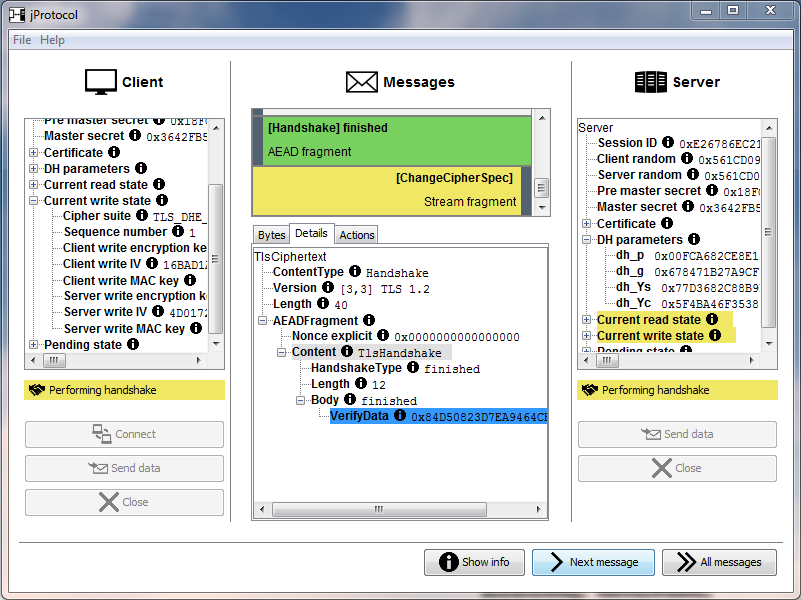
\includegraphics[width=8cm]{pic/ScreenshotTLS.png}
		\end{column}
	\end{columns}
\end{frame}

\begin{frame}[c]{Possible next steps}
	\begin{center}
		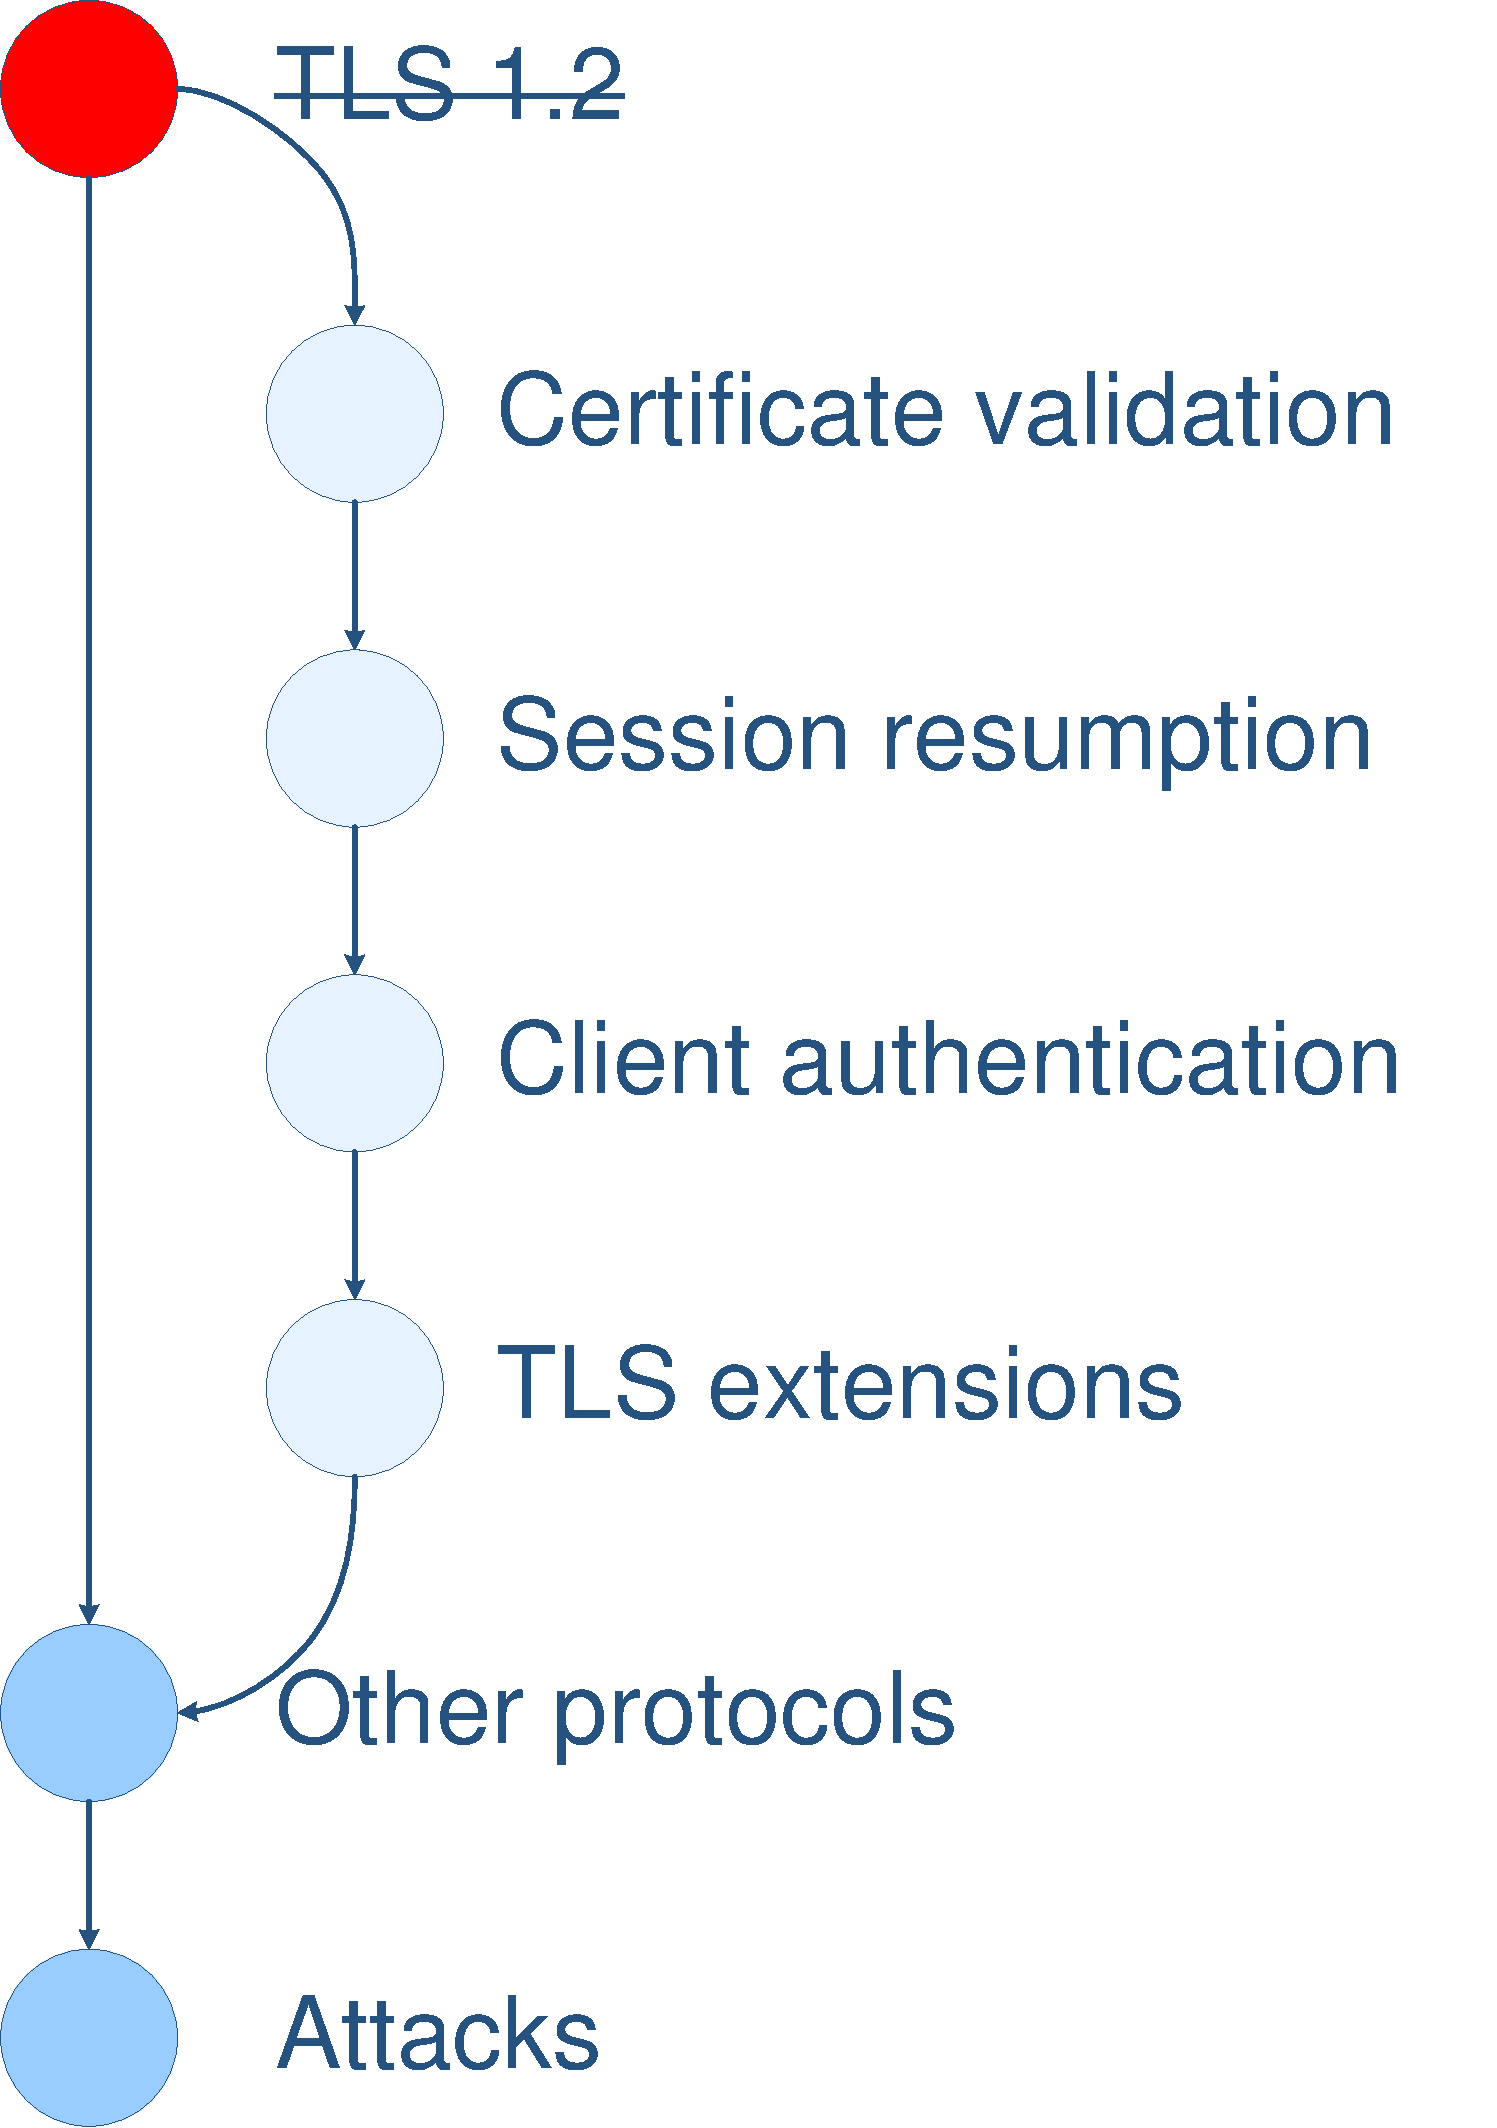
\includegraphics[width=5cm]{pic/TODO.pdf}
	\end{center}
\end{frame}

\begin{frame}[c]{}
\begin{center}
\LARGE Thank you!
\end{center}
\end{frame}

\end{document}